\section{The unique retarded field}
\label{sec:unique-retarded}

A local particular solution is a way to integrate the source at each radius.
The physical boundary conditions are separate. They require the daughter to
propagate into the future horizon and out to infinity, with no incoming
daughter from infinity. We impose these mode limits on the field and its
tortoise derivative. The constants in the incoming parent wave remain fixed.

Let \(u\) be the homogeneous daughter with unit ingoing amplitude at the
horizon, and let \(A_{\mathrm{in}},A_{\mathrm{out}}\) be its amplitudes at
infinity. Write \(w=2k\). At the real physical frequency, the conserved
Wronskian \(W_D(u,\overline u)=2w\) implies
\[
 |A_{\mathrm{in}}|^2-|A_{\mathrm{out}}|^2=1 .
\]
The difference of two solutions with the same source solves the homogeneous
equation. In the basis \(u,\overline u\), the absence of an outgoing horizon
mode forces that difference to equal \(c u\). The absence of an incoming
infinity mode gives \(c A_{\mathrm{in}}=0\). The flux identity makes
\(A_{\mathrm{in}}\) nonzero, so \(c=0\).
This is an exterior uniqueness result at nonzero real frequency. It holds
for any forcing for which a solution has the stated radiation limits.

For each admitted mixture, the regular local field provides one particular
solution. If its incoming coefficient in the scaled projected master is
\(\alpha^2 b_{--}\), subtracting \(\alpha^2 b_{--}u/A_{\mathrm{in}}\)
produces the unique retarded field. This proves the wave solution and the
sign of the subtraction in the boundary expression. The absence of a
homogeneous \emph{rational row} is a second result, at the level of local
coefficients. Its zero-source Laurent bounds leave 18 columns. A nonzero
minor is proportional to
\[
 \ell(3\ell+1)\,[1008 k^2-P(\ell)].
\]
The angular factor is
\[
 \begin{aligned}
 P(\ell)={}&259\ell^8+524\ell^7+134\ell^6-280\ell^5\\
           &-133\ell^4+44\ell^3+28\ell^2 .
 \end{aligned}
\]
Every coefficient of \(P(2+x)\) is positive, and \(k^2<0\).
Consequently each admitted rational row is unique.

\subsection{A Green solution for an arbitrary incident profile}

The classification does not prevent the field for another incident
polarization from having a retarded response. Define
\[
 v=\overline u-\frac{\overline A_{\mathrm{out}}}{A_{\mathrm{in}}}u .
\]
At infinity \(v\) is outgoing, with amplitude \(1/A_{\mathrm{in}}\).
Its Wronskian with \(u\) is \(2w\). For a source \(S\) such that both
integrands are absolutely integrable, the retarded field is
\[
 X_{\rm ret}(r)=\frac{1}{2w}
   \left[
       v(r)\int_2^r \frac{u(s)S(s)}{f(s)}\,\ud s+
       u(r)\int_r^\infty \frac{v(s)S(s)}{f(s)}\,\ud s
   \right].
\]
Differentiation cancels the two moving endpoints in the first derivative,
and the Wronskian produces \(S\) in the second. The same absolute
integrability proves the horizon and infinity mode limits for the field
and its jet. The pure-odd source meets the hypothesis because the ingoing
contraction vanishes at \(r=2\), with \(S/f=O(1)\), and its unscaled radial
coefficients are \(O(r^{-2})\) at infinity. The source and both homogeneous
waves remain bounded after the respective endpoint scalings. The pure-odd
amplitude is a single absolutely convergent integral \(\int_2^\infty
uS/f\) divided by \(2w A_{\mathrm{in}}\).
The two admitted responses and this third response span the full quadratic
dependence on the incident parity coefficients.

\subsection{All azimuthal components of the highest daughter}
\label{sec:angular-followon}

Let \(N=2\ell\), and use even and odd incident polynomials
\[
 A(z)=\sum_{p=0}^N \sqrt{\binom{N}{p}}\,a_{\ell-p} z^p,\qquad
 B(z)=\sum_{p=0}^N \sqrt{\binom{N}{p}}\,b_{\ell-p} z^p.
\]
For the top daughter the Clebsch--Gordan product weight is
\(\sqrt{\binom{N}{p}\binom{N}{q}/\binom{2N}{p+q}}\).
This is the maximal-coupling specialization of the radial and angular
separation in \cite[Sec.~V.4]{bucciotti}. The coefficient of \(z^s\) is
the daughter with \(m=2\ell-s\), after division by the nonzero factor
\(\sqrt{\binom{2N}{s}}\).

The rational obstruction for that daughter is proportional to
\([z^s](B-A)(B-\rho_2 A)\), with \(\rho_2\) from
Theorem~\ref{thm:two}. The whole top multiplet has rational local rows
if and only if \(B=A\) or \(B=\rho_2 A\), because
\(\mathbb{C}[z]\) has no zero divisors.
Even two parent modes that each lie on an admitted branch can create
a cross mode without a rational row. If \(A=z^p+z^q\) and
\(B=z^p+\rho_2 z^q\), the obstruction is
\(-(\rho_2-1)^2z^{p+q}\).

For arbitrary \(A,B\) let
\[
 D(z)=\frac{A(B-A)}{\rho_2-1},\qquad
 C(z)=(B-A)(B-\rho_2 A).
\]
If \(q_1,q_2\) are the common-basis outgoing coefficients of the admitted
mixtures and \(q_{\rm O}\) is the pure-odd integral above, the outgoing
component is
\[
 [z^s]\big((A^2-D)q_1 + Dq_2 + Cq_{\rm O}\big)
\]
with the same angular division. This formula follows by expanding the
three source rows in the common parent basis and using linearity and
uniqueness of the daughter solution.

\section{What the exact responses reveal}
\label{sec:followons}

\subsection{A sign switch in the first low-frequency correction}

The published simulations find leading quadratic scaling in \(M\omega\)
for the studied channels \cite{bucciotti}. Our local formulas make the
first branch-dependent correction accessible.
For the second mixture, the first correction to the leading
frequency-squared-normalized magnitude is negative at \(\ell=2,3,4\) and
positive at every integer \(\ell\ge5\). With \(j\) an angular label the
signed factor is \(d_\ell-2d_{2\ell}\), where
\[
 d_j=\frac{1}{2j+1}
   \left[-2-\frac{4}{j(j+1)}
     +\frac{[(j+1)^2-4]^2}{(2j+1)(2j+2)(2j+3)}
     -\frac{(j^2-4)^2}{(2j-1)(2j)(2j+1)}
   \right].
\]
The linear expansion uses the low-frequency phase and renormalized
angular momentum of \cite{dolan,mst}. The common unit phase cancels from
the magnitude. The positive threshold factor and the sign of the
remaining angular polynomial are separately checked in Lean.
Figure~\ref{fig:soft-sign} supplies two finite-frequency witnesses.
The sign calculation uses the cited linear expansions as premises.
If \(\sigma_\ell\) denotes this slope after division by the leading
coefficient as well as \((M\omega)^2\), then
\(\ell\,\sigma_\ell\to15\pi/16\) in that expansion.

The condition for cancellation of the second admitted strain is more
restrictive at small positive frequency. From the two prefactors,
\[
 Q^-_2=P(k)\big(C(k)R_p^2+R_d\big),\quad
 C(k)=1-\chi+\chi\left(\frac{k-g}{k+g}\right)^2,\quad
 \chi=\frac{(G+g)^2}{4Gg},
\]
where \(g=\gamma_\ell\), \(G=\gamma_{2\ell}/2\), and
\(P(k)=K_\ell k/[4G(k-G)]\) is nonzero.
The squared quotient has unit modulus, so \(C(k)\) traces a circle.
Its modulus exceeds one by a positive quadratic correction near zero.
The loss \(1-|R_p|^2\) is bounded by \(O_\ell((M\omega)^{2\ell+2})\)
using a static positive barrier comparison, consistent with the
published leading absorption law \cite{grayvisser}. Since
\(|R_d|\le1\), the triangle inequality yields
\(|Q^-_2|\ge c_\ell (M\omega)^3>0\) for sufficiently small positive
frequency at every fixed \(\ell\).

\begin{figure}[htbp]
 \centering
 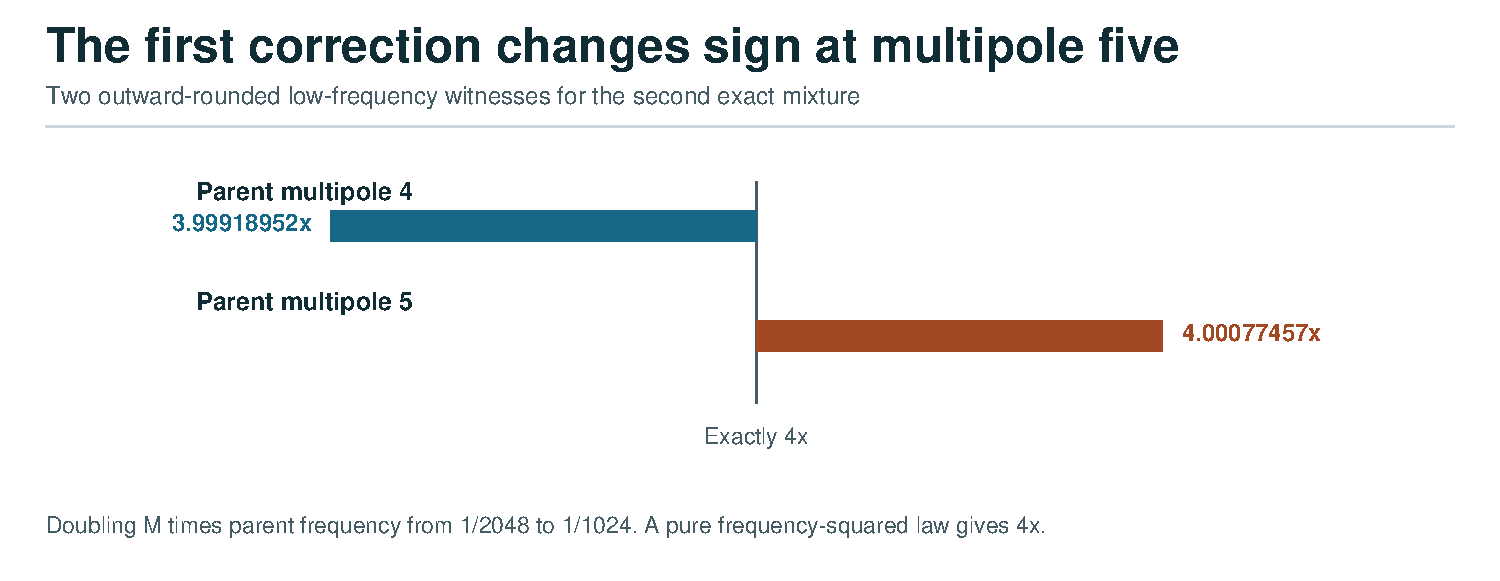
\includegraphics[width=\linewidth]{soft-sign.pdf}
 \caption{A finite-frequency check of the first correction to quadratic
 growth. The second-mixture amplitudes use the incoming-strain convention
 of Section~\ref{sec:strain}. The plotted doubling ratios are rounded
 from outward enclosures. The general sign statement is asymptotic.}
 \label{fig:soft-sign}
\end{figure}

\subsection{A resolved interference dip and two polarization zeros}

At \(\ell=4\) on \(0.650\le M\omega\le 0.675\), interval propagation and
frequency interpolation bound the second admitted response away from
zero on the entire band. Every minimum over that band lies in
\(0.66219<M\omega<0.66565\), with magnitude between
\(1.2130\times10^{-5}\) and \(1.2247\times10^{-5}\).
Exact phase opposition occurs at a lower frequency in
\([0.655,0.660]\), where the two term magnitudes differ by a factor
of at least \(1.00234\). The minimum of the strain magnitude need not
coincide with the crossing of the relative phase.

One may instead change the incident polarization. At the fixed
\(\ell=4,\ M\omega=1/2\) benchmark, write the spin-minus amplitude in
the common parent basis as
\[
 P_-(a,b)=E a^2+Xab+O b^2 .
\]
\begin{figure}[htbp]
 \centering
 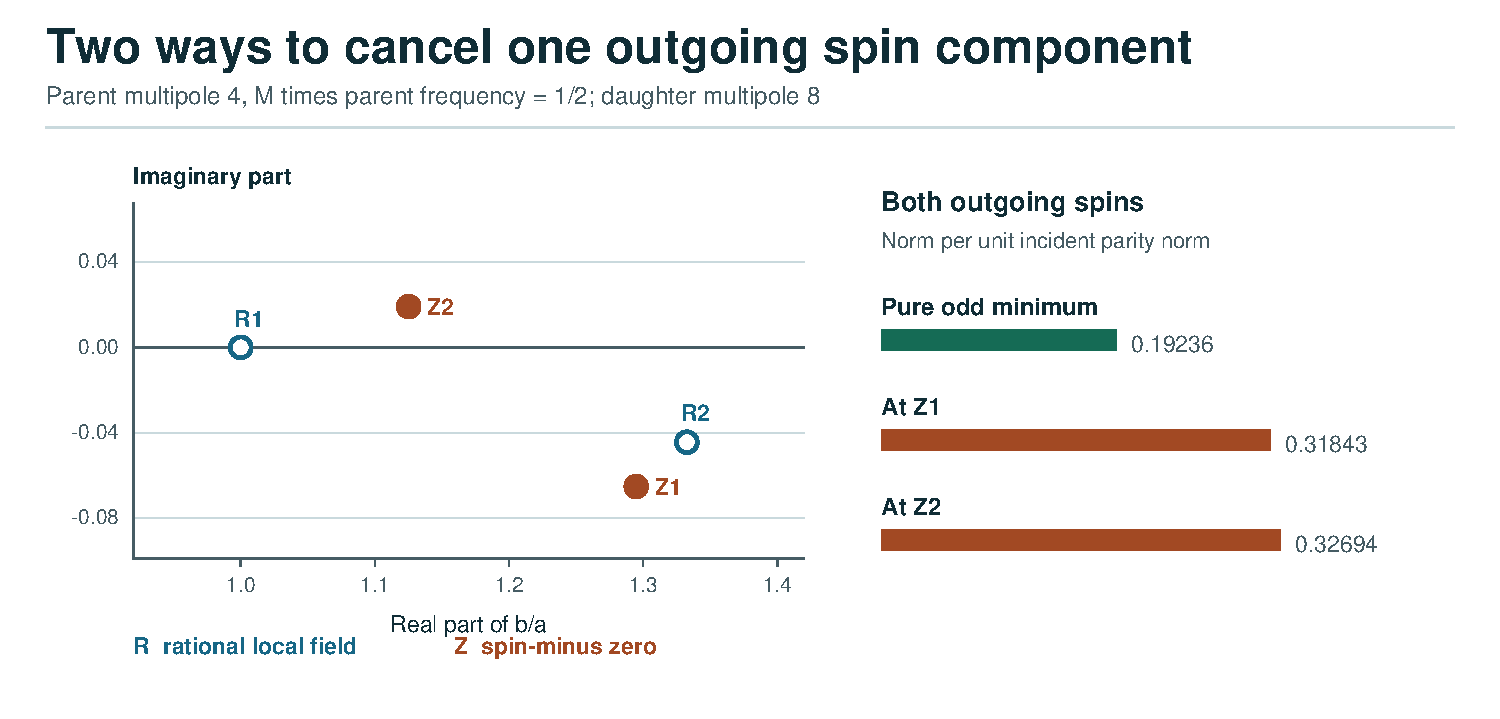
\includegraphics[width=\linewidth]{polarization.pdf}
 \caption{The two rational ratios \(R1,R2\) and the two outgoing
 spin-minus zeros \(Z1,Z2\) are disjoint at the benchmark. The bars
 show the norm of the two outgoing spin amplitudes at fixed unit
 incident parity norm in the common parent basis.}
 \label{fig:polarization}
\end{figure}
We integrate each source component separately on two grids
using the pinned regularized source. Adding the components recovers
both admitted amplitudes and a manufactured source recovers the exact
currents on the horizon, finite interval and infinity pieces.
Direct ball arithmetic isolates two simple roots,
\[
 b/a\simeq 1.294793416343-0.065231726339\,\ii,\qquad
 b/a\simeq 1.125230638044+0.019148752108\,\ii.
\]
Their incident strain normalization is nonzero. Each differs from both
admitted rational ratios. Prior work already found two nearby zeros
under quadrupolar driving \cite[Sec.~V.5, Fig.~6]{bucciotti}. The
result here certifies this fourth-multipole example, links it to the
different rational-local condition, and extends the zero criterion to
all azimuthal modes.

For a general angular profile, \(\mathbb{C}[z]\) has no zero divisors.
The entire top daughter has vanishing spin-minus amplitude exactly when
\(B=\zeta_1 A\) or \(B=\zeta_2 A\), where \(\zeta_i\) are the two roots.
Parity flips only the mixed term for the opposite spin component.
Hence simultaneous vanishing of the two output polynomials would give
\(XAB=0\) and \(EA^2+OB^2=0\). At the benchmark all three coefficients
are nonzero. The only joint zero is zero incident data.
For one incident mode, the half squared output norm is
\[
 |Ea^2+Ob^2|^2+|X|^2 |ab|^2 .
\]
Set \(e=|E|,x=|X|,o=|O|\) and \(t=|a|^2\) with
\(|a|^2+|b|^2=1\). The reverse triangle inequality bounds this by
\(o^2+t[(1-t)(x^2-2o(o+e))+t(e^2-o^2)]\) from below. Both
coefficients inside the brackets are strictly positive in the interval
calculation, so pure odd incidence attains the minimum. Figure~\ref{fig:polarization}
shows that either spin-minus zero leaves a larger total two-spin norm.
The lower bound also gives a floor for arbitrary unit incident profiles.
In the binomial normalization, the squared norm of a polynomial \(P\)
of degree at most \(D\) is
\((D+1)\int |P(z)|^2/(1+|z|^2)^D\,\ud\mu\), with \(\mu\) the
normalized sphere measure. Apply the pointwise scalar lower bound
before integrating and use Jensen's inequality. The daughter norm
is at least \(\sqrt{2(2N+1)}\,o/(N+1)\), about \(0.08812\) in the
common units for \(N=8\). This holds for every unit angular profile,
including profiles with unrelated phases in their two parities.

\subsection{A logarithmically drifting phase at the light ring}

Fix real detuning \(\delta\), with the daughter frequency chosen as
\(2M\omega=(2\ell+\delta)/(3\sqrt3)\), and let \(\ell\) run through
positive integers. Write
\[
 F(b)=\big(1+e^{\pi(2b-1)}\big)^{-1},\quad
 K_0=\frac{5\,2^{1/4}}{36\pi^{3/4}},\quad C_2=\frac{\sqrt3 K_0}{16}.
\]
The first mixture has
\(\ell^{15/4}|Q^-_{1,\ell}|\to 2K_0\sqrt{F(\delta)}\).
The second has a lower and an upper limiting envelope,
\[
 \begin{split}
 \liminf_{\ell\to\infty}\ell^{3/4}|Q^-_{2,\ell}|
   &= C_2\,|F(\delta/2)-\sqrt{F(\delta)}|,\\
 \limsup_{\ell\to\infty}\ell^{3/4}|Q^-_{2,\ell}|
   &= C_2\,[F(\delta/2)+\sqrt{F(\delta)}].
 \end{split}
\]
The two contributions settle in modulus on this scale while their
relative phase keeps changing. Its leading form is
\(\tfrac12\log\ell+\theta(\delta)+o(1)\) modulo \(2\pi\).
It is invariant under translation of the tortoise-coordinate origin
because the frequencies add exactly.

The matching uses the Weber barrier-top connection, as in the linear
semiclassical problem \cite{ramond,dlmf}. Specifically let
\(h=(j+1/2)^{-1}\) for an individual linear wave and use
\(M w_{\rm lin}=(j+b)/(3\sqrt3)\).
Near \(r=3\), \(V_0=f/r^2\) has a nondegenerate maximum
\(a=1/27\) in the \(M=1\) convention. After the scaling \(x=\sqrt h\,y\)
the leading equation is
\[
 U''+(a^2 y^2+2a(b-1/2))\,U=0 .
\]
Matching at \(x=\pm h^{2/5}\) gives a coefficient error
\(O(h^{1/5})\) at fixed detuning. The inner remainder integrates as
\(O(\sqrt h Y^3+h\log(1+Y))\) with \(Y=h^{-1/10}\) in the Weber
basis. On the exterior the WKB error is controlled by
\(O(h\,h^{-4/5})\) at the cut and by integrable tails. The
linear phase includes \((b-1/2)\log(j+1/2)\).
In \(R_d/R_p^2\), its logarithmic coefficient is
\((\delta-1/2)-2(\delta/2-1/2)=1/2\).
The global action terms leave a constant, and the parent Darboux
phase tends to one. The full matching, including the exterior
phase constants, is supplied with the source.

\begin{figure}[htbp]
 \centering
 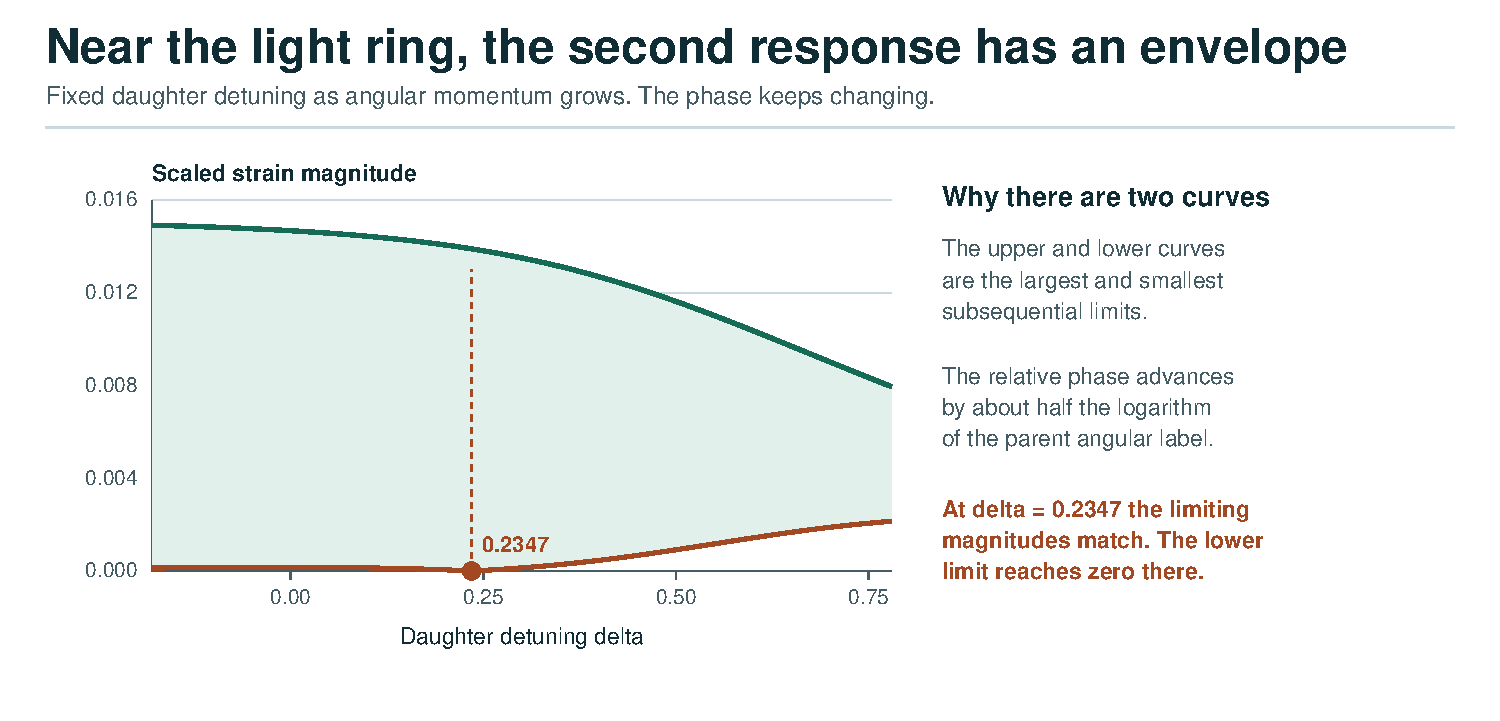
\includegraphics[width=\linewidth]{light-ring.pdf}
 \caption{The second-mixture light-ring limits. Fixed detuning
 \(\delta\) is measured relative to the leading daughter frequency.
 The lower limit reaches zero only at the limiting magnitude
 balance. It is attained along subsequences with increasing \(\ell\).}
 \label{fig:light-ring}
\end{figure}

Integer labels nearest to
\(\exp(2(2\pi m+\varphi-\theta))\) realize any relative phase
\(\varphi\) in the limit. This gives both envelopes. They balance at
\(\delta_\ast = 1+\pi^{-1}\log(2/(e^\pi-1))\simeq0.23469708\),
where a subsequence of the scaled magnitude approaches zero. The
statement concerns the limit, and leaves open exact finite-label zeros
along these two admitted branches and the separate pure-even eikonal
question of \cite[Sec.~V.3]{bucciotti}.
Lean checks the envelope and phase-subsequence argument from the
linear matching hypotheses. Numerical controls use different
propagators and extraction methods to check the analytic phase.
